\chapter{Resolver Workflows}\label{sec:resolver-workflows}

\section{Overview}
For any scan invoked by \cxoneflow\space when \intlink{sec:scan-agent-elements}{configured to use a scan agent,} 
a delegated scan is enqueued with the message queue to run a resolver scan and/or a pre-scan script.  The delegated scan is handed over
to a Scan Agent that clones the code and executes \scaresolver.  The \scaresolver results are
then submitted for scan along with the code.  The executing scan then follows any configured feedback workflows.
This section details exchange, queue, and workflow logic of this process.


\section{Delegated Scan Workflow}

The \cxoneflow endpoint logs will indicate scans are delegated when the algorithm for event handling
determines a resolver or pre-scan script should be executed.  Figure \ref{fig:delegated-scan-flowchart} shows the delegated scan
workflow algorithm that is followed to determine when to request a delegated scan.  


\begin{figure}[ht]
  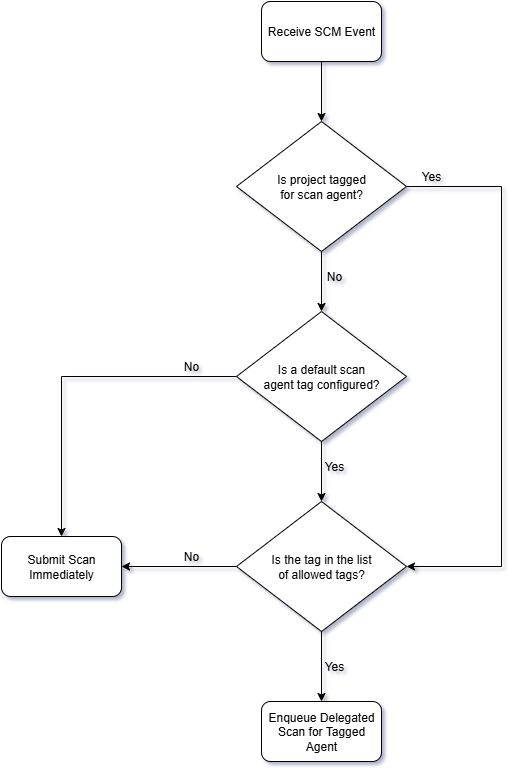
\includegraphics[scale=.8]{graphics/cxoneflow-diagrams-Delegated Scan Algorithm.png}
  \centering
  \caption{Delegated Scan Algorithm}
  \label{fig:delegated-scan-flowchart}
\end{figure}


\section{Post Delegated Scan Workflow}

When the \scaresolver scan and/or pre-scan script is complete, the Scan Agent will submit
a scan request following the service endpoint configuration.  The data for the running scan
is then published for handling by any workflow agents that perform workflows when the
scan is complete (e.g. Pull request decorations).  These scan steps can
complete successfully or end with failure.  Even if any of the pre-scan steps ends in 
failure, the scan is submitted.

If the \scaresolver scan is successful, the results of the 
\extlink{https://docs.checkmarx.com/en/34965-19199-running-scans-using-checkmarx-sca-resolver.html\#UUID-af718204-6dfc-2b27-439e-419b9157d364_id_RunningScansUsingCheckmarxSCAResolver-CheckmarxSCAResolverModes}{offline}
scan are submitted as part of the \cxone scan.  If the \scaresolver scan fails (for any reason), the \cxone scan is submitted for server-side dependency resolution.
Figure \ref{fig:post-delegated-scan-flowchart} shows the post-delegated-scan workflow algorithm.

\begin{figure}[ht]
  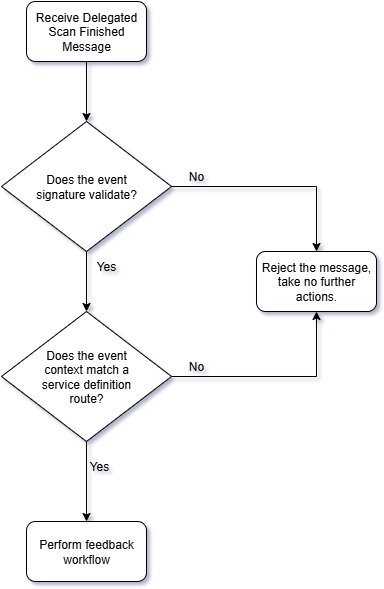
\includegraphics[scale=.8]{graphics/cxoneflow-diagrams-Post Delegated Scan Algorithm.png}
  \centering
  \caption{Post Delegated Scan Algorithm}
  \label{fig:post-delegated-scan-flowchart}
\end{figure}



